\documentclass{beamer}

\usepackage{polyglossia}
\setmainlanguage{russian}
\setotherlanguage{english}
\defaultfontfeatures{Ligatures={Common,TeX}}
\setromanfont{CMU Serif}
\setsansfont{CMU Sans Serif}
\setmonofont{CMU Typewriter Text}

\usepackage{graphicx}

\hypersetup{pdfstartview={Fit}}

\title[Машинная графика]{Курсовая работа по ``Машинной графике''}
\subtitle{Симулятор детского конструктора}
\author{Студент: {Амиантов Николай Ильич, ИУ7-52}, \\
Научный руководитель: {Ломовской Игорь Владимирович}}
\date{\today}

\begin{document}

\frame{\titlepage}

\begin{frame}
\frametitle{Возможности}

\begin{itemize}
\item Добавление, удаление объектов со сцены
\item Модели произвольны, загружаются из файлы
\item Отрисовка сцены с большим количеством настроек растеризатора
\item Редактирование сцены --- перенос, поворот объектов
\item Сохранение и загрузка сцены
\item Освещение сцены
\item Все настройки --- в файлах
\end{itemize}
\end{frame}

\begin{frame}
\frametitle{Основные задачи}

\begin{itemize}
\item Растеризация
\item Загрузка моделей
\item Редактирование сцены
\item Загрузка и сохранение сцены
\end{itemize}
А также реализация, тестирование и интенсивная оптимизация всего вышеперечисленного.
\end{frame}

\begin{frame}
\frametitle{Схожие продукты}
\framesubtitle{Garry's Mod}

\centering
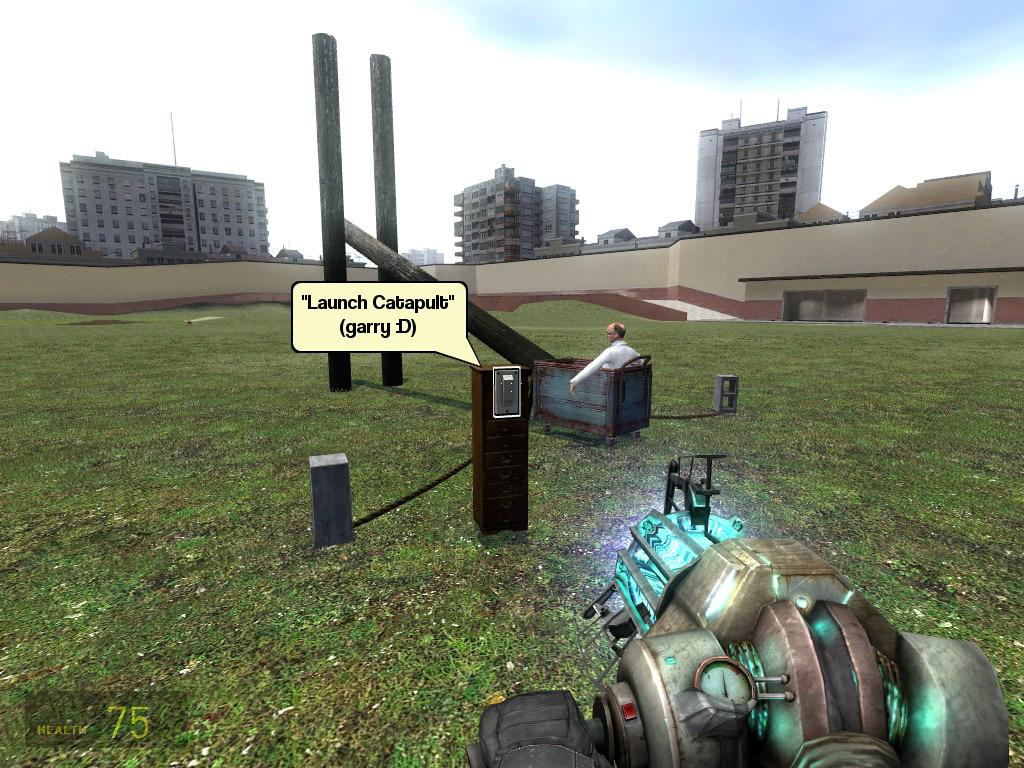
\includegraphics[width=\textwidth]{garrysmod}
\end{frame}

\begin{frame}
\frametitle{Представление моделей}

\begin{itemize}
\item Полигональное \\
Простая, быстрая, экономичная по памяти модель
\item Воксельное \\
Реалистичная модель с возможностью изменения в реальном времени
\end{itemize}
Нужна скорость --- полигональное представление.
\end{frame}

\begin{frame}
\frametitle{Удаление невидимых линий}

\begin{itemize}
\item Алгоритм Робертса \\
Точный, медленный, сложный
\item Алгоритм Вейлера-Азертона \\
Быстр на простых сценах, рекурсивный
\item Z-буферизация \\
Простой, быстрый на современных машинах
\end{itemize}
Выберем Z-буферизацию из-за скорости
\end{frame}

\begin{frame}
\frametitle{Модели освещения}

\begin{itemize}
\item Модель Кука-Торренса \\
Бликовое освещение, точный, медленный
\item Модель Ламберта \\
Простая, описывает диффузное освещение
\item Модель Фонга \\
Эмпирическая, относительно быстрая
\item Модель Блинна-Фонга \\
Точный для разных материалов, медленее чем Фонг
\end{itemize}
Для скорости выбрали модель Фонга
\end{frame}

\begin{frame}
\frametitle{Векторы и матрицы}

\begin{itemize}
\item Храним в массивах
\item Афинные преобразования --- матрицы 3х4 достаточно
\item Реализованы алгоритмы вычисления углов, извлечения эйлеровых координат и.т.д.
\item Перспективное преобразование реализовано отдельно, не матрицей
\end{itemize}
\end{frame}

\begin{frame}
\frametitle{Хранение моделей}
\framesubtitle{Хранение точек}

\begin{itemize}
\item Точки массивом \\
Экономично, быстро, неэффективно если точки меняются
\item Точки списком \\
Медленнее но быстрее добавление/удаление
\item BSP-дерево \\
Специальное дерево, медленно если объект движется
\end{itemize}
Точки не будут меняться --- выберем массив.
\end{frame}

\begin{frame}
\frametitle{Хранение моделей}
\framesubtitle{Многоугольники}

\begin{itemize}
\item Хранить многоугольники --- требуется обрабатывать случаи невыпуклости
\item Треугольники --- однозначно задают плоскость, не требуют проверок
\item В графических библиотеках используются треугольники
\end{itemize}
Выберем треугольники.
\end{frame}

\begin{frame}
\frametitle{Хранение моделей}
\framesubtitle{Хранение треугольников}

\begin{itemize}
\item Хранить как наборы точек \\
Частые повторы.
\item Хранить как наборы индексов в общем массиве точек \\
Значительно экономичнее, чуть медленнее. Используется в графических библиотеках.
\end{itemize}
Будем хранить наборами индексов.
\end{frame}

\begin{frame}
\frametitle{Хранение моделей}
\framesubtitle{Что ещё нужно хранить}

\begin{itemize}
\item Нормали к вершинам --- получаем из файла
\item Нормали к сторонам --- высчитываем векторным произведением.
\item Материал для каждой стороны.
\item UV-координаты.
\end{itemize}
\end{frame}

\begin{frame}
\frametitle{Материал}

\begin{itemize}
\item Храним параметры для освещения по выбранной модели
\item Возможно, текстуру
\item Текстура --- подгружается и конвертируется в формат экрана
\item Несколько сторон могут использовать один экземпляр материала
\item Материал также может исключать сторону из расчёта освещения
\end{itemize}
\end{frame}

\begin{frame}
\frametitle{Объект на сцене}
\framesubtitle{Структура данных}

\begin{itemize}
\item Храним ссылку на модель
\item Положение объектов на экране
\item Кэшированные преобразованные точки
\item Оверлей материалов
\end{itemize}
\end{frame}

\begin{frame}
\frametitle{Объект на сцене}
\framesubtitle{Позиция}

\begin{itemize}
\item Хранить матрицей \\
Неудобно для редактирования пользователем
\item Хранить эйлеровыми углами и начальной точкой \\
Не всегда удобно для преобразований, но удобно для пользователя.
\end{itemize}
Выберем второй вариант --- пользователь сможет удобно задавать позиции.
\end{frame}

\begin{frame}
\frametitle{Объект на сцене}
\framesubtitle{Источник света}

\begin{itemize}
\item Объект может быть источником света
\item В таком случае хранит параметры для модели освещения
\item Параметры могут быть индивидуальны для каждого объекта
\item Они хранятся в описании сцены
\end{itemize}
\end{frame}

\begin{frame}
\frametitle{Объект на сцене}
\framesubtitle{Кэш}

\begin{itemize}
\item Объект задаётся моделью и позицией
\item Каждый раз преобразовывать точки модели в мировую СК --- медленно
\item Позиция объекта меняется не так часто
\item Будем хранить результаты преобразований
\end{itemize}
\end{frame}

\begin{frame}
\frametitle{Объект на сцене}
\framesubtitle{Оверлей материалов}

\begin{itemize}
\item Хотим заменить у конкретного объекта материал конкретной стороны
\item Будем хранить словарь ``номер вершины --- новый материал''
\item Словарь пополняется со стороны
\end{itemize}
\end{frame}

\begin{frame}
\frametitle{Сцена}

\begin{itemize}
\item Поскольку не используем BSP-дерево, храним просто множество объектов
\item Массив \\
Медленный для изменения количества
\item Связный список \\
Медленнее массива, но быстрое добавление/удаление
\end{itemize}
Предполагается добавление/удаление объектов --- будем использовать связный список.
\end{frame}

\begin{frame}
\frametitle{Отрисовка}
\framesubtitle{Камера}

\begin{itemize}
\item Храним камеру также как позицию объекта
\item Переводим точки в её систему координат
\item Камера также хранит настройки для перспективного преобразования
\item Управляется с помощью кнопок клавиатуры
\end{itemize}
\end{frame}

\begin{frame}
\frametitle{Отрисовка}
\framesubtitle{Источники света}

\begin{itemize}
\item Каждый объект может быть источником света
\item Перед преобразованиями создаётся массив параметров источников
\item Для уменьшения количества выделений памяти массив сохраняется между кадрами
\item Используется во время преобразований для определения параметров освещения точек
\end{itemize}
\end{frame}

\begin{frame}
\frametitle{Отрисовка}
\framesubtitle{Кэш точек}

\begin{itemize}
\item Необходимо хранить преобразованные точки
\item Выделять память каждый кадр --- маедленно
\item Будем хранить между кадрами аллоцированную память для точек и пр.
\end{itemize}
\end{frame}

\begin{frame}
\frametitle{Отрисовка}
\framesubtitle{Отсечение по направлению грани}

\begin{itemize}
\item Часть выпуклого объекта всегда заслонена от наблюдателя
\item Можно не отрисовывать то, что не может быть видимо
\item Определяем по направлению нормали к грани и направлению камеры
\end{itemize}
\end{frame}

\begin{frame}
\frametitle{Отрисовка}
\framesubtitle{Отсечение по плоскостям}

\begin{itemize}
\item Проверять, находится ли каждый пиксель в границах экрана --- сильно замедляет работу
\item Делать простое отсечение по прямоугольнику, закрашивать с проверкой то что целиком внутри --- быстрее
\item Делать полное отсечение --- самый быстрый вариант для общего случая
\end{itemize}
Реализовано полное отсечение с упрощениями для треугольников.
\end{frame}

\begin{frame}
\frametitle{Отрисовка}
\framesubtitle{Билинейная интерполяция}

\begin{itemize}
\item Используется для глубины, UV-координат и других величин.
\item Реализованы общие алгоритмы обхода
\item Нужная операция ``собирается'' из классов, описывающих простые типы и методы их интерполяции
\item Используется шаблонное метапрограммирование
\end{itemize}
\end{frame}

\begin{frame}
\frametitle{Отрисовка}
\framesubtitle{Интерполяция текстур}

\begin{itemize}
\item Можно интерполировать координаты афинно \\
Создаёт артефакты на наклонённых плоскостях
\item Перспективная интерполяция \\
Учитывает перспективу, тяжелее для расчёта
\end{itemize}
Реализованы оба метода, проведено сравнение
\end{frame}

\begin{frame}
\frametitle{Отслеживание взгляда пользователя}

\begin{itemize}
\item Необходимо для редактирования сцены
\item Реализуется через оптимизированный алгоритм обхода треугольника
\item У отслеженной стороны изменяется материал чтобы показать пользователю, на какую сторону он смотрит
\item Реализовано через оверлей материалов
\end{itemize}
\end{frame}

\begin{frame}
\frametitle{Операции над телами}

\begin{itemize}
\item Влечение за камерой \\
Удобное перемещение объектов
\item Поворот относительно точки \\
Интуитивный поворот тел относительно осей камеры
\item Перенос к другому телу \\
Элемент ``конструирования'', совмещение объектов.
\end{itemize}
\end{frame}

\begin{frame}
\frametitle{Загрузка/сохранение данных}
\framesubtitle{Общий формат данных}

\begin{itemize}
\item Свой формат --- зачем изобретать велосипед?
\item XML --- 50\% текста --- управляющие структуры, ужасно выглядит.
\item YAML --- чёткая структура, максимум данных и выразительности.
\end{itemize}
Выберем YAML для хранения данных
\end{frame}

\begin{frame}
\frametitle{Загрузка/сохранение данных}
\framesubtitle{Формат данных моделей}

\begin{itemize}
\item Свой формат --- опять же, зачем?
\item Wavefront OBJ --- простой, однако функциональный
\item Object File Format --- самый примитивный, минимум структур
\item DirectX Model Format --- иерархический, выразительный но простой для редактирования, распостранённый
\item COLLADA/X3D --- основаны на XML, и это недостаток
\end{itemize}
Был выбран DirectX Model Format --- было сложно реализовать, однако он удобен.
\end{frame}

\begin{frame}
\frametitle{Язык программирования}

\begin{itemize}
\item Приоритет скорости (как в C)
\item Тем не менее, функциональность имеет значение
\item Выбран C++ --- код близок по скорости к C, однако есть поддержка ООП
\item Как бонус --- множество библиотек на все случаи жизни
\end{itemize}
\end{frame}

\begin{frame}
\frametitle{Сторонние библиотеки и утилиты}

\begin{itemize}
\item C++ STL --- встроенная библиотека C++ --- структуры данных и алгоритмы
\item SDL --- основная библиотека интерфейса и отрисовки
\item flex/bison --- генераторы синтаксических и лексических анализаторов, для парсера .x
\item Boost --- форматирование текста, файловая система и дата/время
\item Eigen3 --- сторонная библиотека работы над векторами и матрицами, используется опционально
\item yaml4cpp --- реализация парсера/построителя YAML
\end{itemize}
\end{frame}

\begin{frame}
\frametitle{Особенности разработки}

\begin{itemize}
\item Изучался стандарт C++11
\item Изучалась теория лексических анализаторов, flex/bison
\item Большая избыточность --- код предполагается использовать в другом проекте
\item Продумывалась общая архитектура конвейера, игрового интерфейса и элементов управления
\item Выделение общих кусков кода в библиотеки для последующего использования
\end{itemize}
\end{frame}

\begin{frame}
\frametitle{Конфигурирование программы}

\begin{itemize}
\item Во время компиляции --- отключение/включение оптимизаций и возможностей рендерера
  \begin{itemize}
  \item Реализовано через макросы
  \item Каждый вариант сборки оптимизирован индивидуально --- максимальная скорость для всех случаев
  \item Шаблонное метапрограммирование
  \end{itemize}
\item Во время исполнения --- размер окна, шрифт, чувствительность мыши и пр.
  \begin{itemize}
  \item Настройки загружаются во время запуска программы
  \item Не могут быть изменены в программе
  \item Формат настроек удобен и человекочитаем
  \end{itemize}
\end{itemize}
\end{frame}

\begin{frame}
\frametitle{Отдельные библиотеки}

\begin{itemize}
\item sdlobj --- ООП-обёртка над SDL
\item xparse --- парсер файлов .x
\item settings --- чтение и применение настроек ко всем модулям программы
\item logging --- сборка и сохранение логов со всей программы
\item common --- библиотека общих алгоритмов и паттернов
\end{itemize}
Всё это --- код на будущее
\end{frame}

\begin{frame}
\frametitle{Архитектура программы}

\begin{itemize}
\item Максимальная модульность
\item Большая универсальность
\item Расширяемость на будущее
\item Структурность
\end{itemize}
Подробности описаны в РПЗ
\end{frame}

\begin{frame}
\frametitle{Интерфейс}

\begin{itemize}
\item SDL не предоставляет своих элементов управления, лишь окно
\item Была написана библиотека элементов управления --- кнопки, текстовые поля, текстовые метки и пр.
\item Интерфейс --- смесь горячих клавиш и динамически возникающих элементов управления
\end{itemize}
\end{frame}

\begin{frame}
\frametitle{Исследования}
\framesubtitle{Что можно было сравнить}

\begin{itemize}
\item Оптимизации компилятора
\item Сравнение библиотек работы с матрицами и векторами
\item Наличие/отсутствие отсечения по нормалям
\item Сравнение методов тонирования
\item Сравнение методов интерполяции текстурных координат
\end{itemize}
\end{frame}

\begin{frame}
\frametitle{Исследования}
\framesubtitle{Результаты}

\begin{itemize}
\item Оптимизации компилятора имеют большое значение
\item Использование векторных инструкций процессора даёт большой прирост скорости
\item Перспективное отсечение по нормалям --- оптимально
\item Тонирование по Гуро --- хорошее качество, приемлемая скорость
\item Перспективная интерполяция --- небольшое замедление, лучше качество
\end{itemize}
Подробности --- в РПЗ.
\end{frame}

\begin{frame}
\frametitle{Внешний вид}

\centering
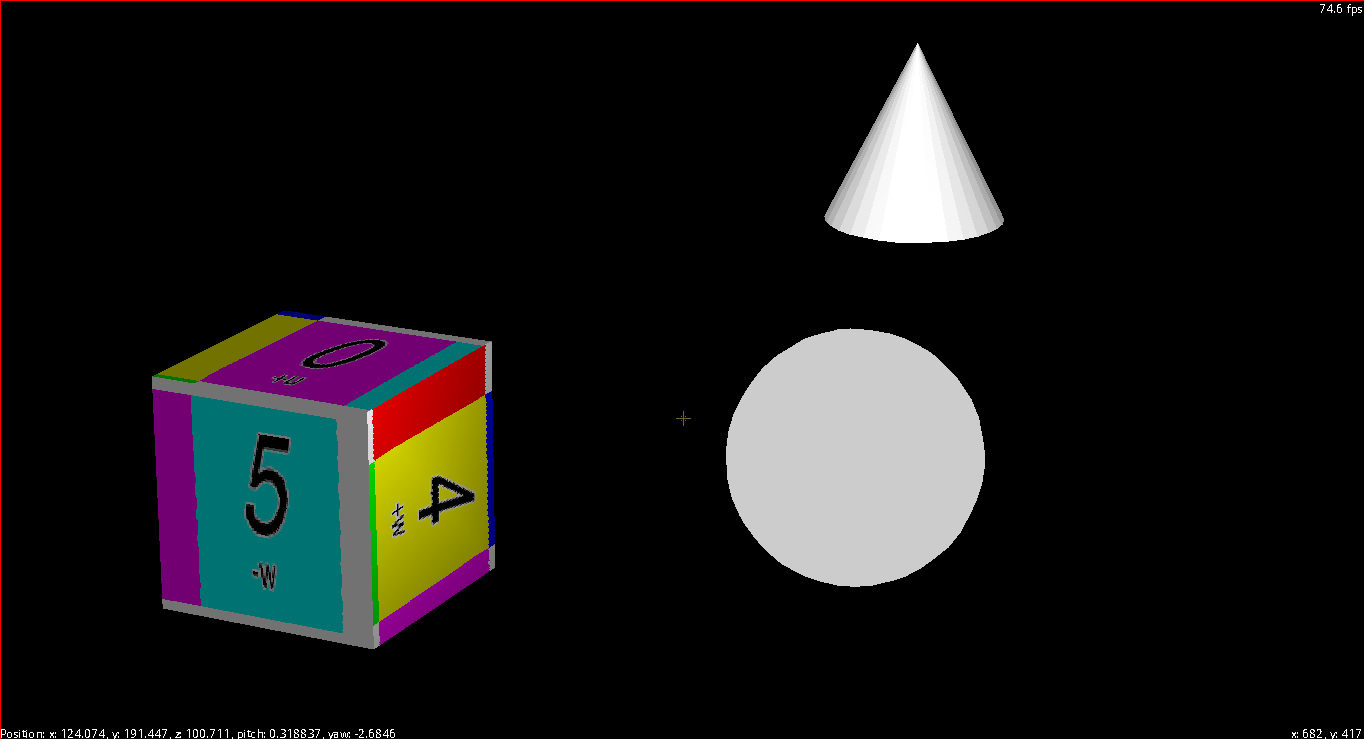
\includegraphics[width=\textwidth]{window}
\end{frame}

\begin{frame}
\centering
Спасибо за внимание!
\end{frame}

\end{document}